% Options for packages loaded elsewhere
\PassOptionsToPackage{unicode}{hyperref}
\PassOptionsToPackage{hyphens}{url}
\PassOptionsToPackage{dvipsnames,svgnames,x11names}{xcolor}
%
\documentclass[
  a4paper,
  DIV=11,
  numbers=noendperiod]{scrartcl}

\usepackage{amsmath,amssymb}
\usepackage{iftex}
\ifPDFTeX
  \usepackage[T1]{fontenc}
  \usepackage[utf8]{inputenc}
  \usepackage{textcomp} % provide euro and other symbols
\else % if luatex or xetex
  \usepackage{unicode-math}
  \defaultfontfeatures{Scale=MatchLowercase}
  \defaultfontfeatures[\rmfamily]{Ligatures=TeX,Scale=1}
\fi
\usepackage{lmodern}
\ifPDFTeX\else  
    % xetex/luatex font selection
\fi
% Use upquote if available, for straight quotes in verbatim environments
\IfFileExists{upquote.sty}{\usepackage{upquote}}{}
\IfFileExists{microtype.sty}{% use microtype if available
  \usepackage[]{microtype}
  \UseMicrotypeSet[protrusion]{basicmath} % disable protrusion for tt fonts
}{}
\makeatletter
\@ifundefined{KOMAClassName}{% if non-KOMA class
  \IfFileExists{parskip.sty}{%
    \usepackage{parskip}
  }{% else
    \setlength{\parindent}{0pt}
    \setlength{\parskip}{6pt plus 2pt minus 1pt}}
}{% if KOMA class
  \KOMAoptions{parskip=half}}
\makeatother
\usepackage{xcolor}
\usepackage[inner=2.5cm,outer=2.5cm,top=3cm,bottom=4cm,headsep=22pt,headheight=11pt,footskip=33pt,ignorehead,ignorefoot,heightrounded]{geometry}
\setlength{\emergencystretch}{3em} % prevent overfull lines
\setcounter{secnumdepth}{5}
% Make \paragraph and \subparagraph free-standing
\makeatletter
\ifx\paragraph\undefined\else
  \let\oldparagraph\paragraph
  \renewcommand{\paragraph}{
    \@ifstar
      \xxxParagraphStar
      \xxxParagraphNoStar
  }
  \newcommand{\xxxParagraphStar}[1]{\oldparagraph*{#1}\mbox{}}
  \newcommand{\xxxParagraphNoStar}[1]{\oldparagraph{#1}\mbox{}}
\fi
\ifx\subparagraph\undefined\else
  \let\oldsubparagraph\subparagraph
  \renewcommand{\subparagraph}{
    \@ifstar
      \xxxSubParagraphStar
      \xxxSubParagraphNoStar
  }
  \newcommand{\xxxSubParagraphStar}[1]{\oldsubparagraph*{#1}\mbox{}}
  \newcommand{\xxxSubParagraphNoStar}[1]{\oldsubparagraph{#1}\mbox{}}
\fi
\makeatother


\providecommand{\tightlist}{%
  \setlength{\itemsep}{0pt}\setlength{\parskip}{0pt}}\usepackage{longtable,booktabs,array}
\usepackage{calc} % for calculating minipage widths
% Correct order of tables after \paragraph or \subparagraph
\usepackage{etoolbox}
\makeatletter
\patchcmd\longtable{\par}{\if@noskipsec\mbox{}\fi\par}{}{}
\makeatother
% Allow footnotes in longtable head/foot
\IfFileExists{footnotehyper.sty}{\usepackage{footnotehyper}}{\usepackage{footnote}}
\makesavenoteenv{longtable}
\usepackage{graphicx}
\makeatletter
\def\maxwidth{\ifdim\Gin@nat@width>\linewidth\linewidth\else\Gin@nat@width\fi}
\def\maxheight{\ifdim\Gin@nat@height>\textheight\textheight\else\Gin@nat@height\fi}
\makeatother
% Scale images if necessary, so that they will not overflow the page
% margins by default, and it is still possible to overwrite the defaults
% using explicit options in \includegraphics[width, height, ...]{}
\setkeys{Gin}{width=\maxwidth,height=\maxheight,keepaspectratio}
% Set default figure placement to htbp
\makeatletter
\def\fps@figure{htbp}
\makeatother
% definitions for citeproc citations
\NewDocumentCommand\citeproctext{}{}
\NewDocumentCommand\citeproc{mm}{%
  \begingroup\def\citeproctext{#2}\cite{#1}\endgroup}
\makeatletter
 % allow citations to break across lines
 \let\@cite@ofmt\@firstofone
 % avoid brackets around text for \cite:
 \def\@biblabel#1{}
 \def\@cite#1#2{{#1\if@tempswa , #2\fi}}
\makeatother
\newlength{\cslhangindent}
\setlength{\cslhangindent}{1.5em}
\newlength{\csllabelwidth}
\setlength{\csllabelwidth}{3em}
\newenvironment{CSLReferences}[2] % #1 hanging-indent, #2 entry-spacing
 {\begin{list}{}{%
  \setlength{\itemindent}{0pt}
  \setlength{\leftmargin}{0pt}
  \setlength{\parsep}{0pt}
  % turn on hanging indent if param 1 is 1
  \ifodd #1
   \setlength{\leftmargin}{\cslhangindent}
   \setlength{\itemindent}{-1\cslhangindent}
  \fi
  % set entry spacing
  \setlength{\itemsep}{#2\baselineskip}}}
 {\end{list}}
\usepackage{calc}
\newcommand{\CSLBlock}[1]{\hfill\break\parbox[t]{\linewidth}{\strut\ignorespaces#1\strut}}
\newcommand{\CSLLeftMargin}[1]{\parbox[t]{\csllabelwidth}{\strut#1\strut}}
\newcommand{\CSLRightInline}[1]{\parbox[t]{\linewidth - \csllabelwidth}{\strut#1\strut}}
\newcommand{\CSLIndent}[1]{\hspace{\cslhangindent}#1}

\KOMAoption{captions}{tableheading}
\makeatletter
\@ifpackageloaded{tcolorbox}{}{\usepackage[skins,breakable]{tcolorbox}}
\@ifpackageloaded{fontawesome5}{}{\usepackage{fontawesome5}}
\definecolor{quarto-callout-color}{HTML}{909090}
\definecolor{quarto-callout-note-color}{HTML}{0758E5}
\definecolor{quarto-callout-important-color}{HTML}{CC1914}
\definecolor{quarto-callout-warning-color}{HTML}{EB9113}
\definecolor{quarto-callout-tip-color}{HTML}{00A047}
\definecolor{quarto-callout-caution-color}{HTML}{FC5300}
\definecolor{quarto-callout-color-frame}{HTML}{acacac}
\definecolor{quarto-callout-note-color-frame}{HTML}{4582ec}
\definecolor{quarto-callout-important-color-frame}{HTML}{d9534f}
\definecolor{quarto-callout-warning-color-frame}{HTML}{f0ad4e}
\definecolor{quarto-callout-tip-color-frame}{HTML}{02b875}
\definecolor{quarto-callout-caution-color-frame}{HTML}{fd7e14}
\makeatother
\makeatletter
\@ifpackageloaded{caption}{}{\usepackage{caption}}
\AtBeginDocument{%
\ifdefined\contentsname
  \renewcommand*\contentsname{Table of contents}
\else
  \newcommand\contentsname{Table of contents}
\fi
\ifdefined\listfigurename
  \renewcommand*\listfigurename{List of Figures}
\else
  \newcommand\listfigurename{List of Figures}
\fi
\ifdefined\listtablename
  \renewcommand*\listtablename{List of Tables}
\else
  \newcommand\listtablename{List of Tables}
\fi
\ifdefined\figurename
  \renewcommand*\figurename{Figure}
\else
  \newcommand\figurename{Figure}
\fi
\ifdefined\tablename
  \renewcommand*\tablename{Table}
\else
  \newcommand\tablename{Table}
\fi
}
\@ifpackageloaded{float}{}{\usepackage{float}}
\floatstyle{ruled}
\@ifundefined{c@chapter}{\newfloat{codelisting}{h}{lop}}{\newfloat{codelisting}{h}{lop}[chapter]}
\floatname{codelisting}{Listing}
\newcommand*\listoflistings{\listof{codelisting}{List of Listings}}
\makeatother
\makeatletter
\makeatother
\makeatletter
\@ifpackageloaded{caption}{}{\usepackage{caption}}
\@ifpackageloaded{subcaption}{}{\usepackage{subcaption}}
\makeatother

\ifLuaTeX
  \usepackage{selnolig}  % disable illegal ligatures
\fi
\usepackage{bookmark}

\IfFileExists{xurl.sty}{\usepackage{xurl}}{} % add URL line breaks if available
\urlstyle{same} % disable monospaced font for URLs
\hypersetup{
  pdftitle={EPRI Grid Forming},
  pdfauthor={Nils Wiese (Fraunhofer IEE); Martin Franke (Fraunhofer IEE); Saikrishna Vallabhaneni},
  colorlinks=true,
  linkcolor={blue},
  filecolor={Maroon},
  citecolor={Blue},
  urlcolor={Blue},
  pdfcreator={LaTeX via pandoc}}


\title{EPRI Grid Forming}
\author{Nils Wiese (Fraunhofer IEE) \and Martin Franke (Fraunhofer
IEE) \and Saikrishna Vallabhaneni}
\date{}

\begin{document}
\maketitle

\renewcommand*\contentsname{Table of contents}
{
\hypersetup{linkcolor=}
\setcounter{tocdepth}{3}
\tableofcontents
}
\listoffigures
\listoftables

\section{Context}\label{context}

This model was developped by Electric Power Research Institute (EPRI)
and provides a standarized approch for inverter based resources {[}1{]}.
The orignal model is described in a PDF available on the
\href{https://www.epri.com/research/products/000000003002021403}{webpage}.

\section{Model use, assumptions, validity domain and
limitations}\label{model-use-assumptions-validity-domain-and-limitations}

The model is a positive-sequence RMS model, hence it assumes symmetrical
operating conditions and neglects high-frequency dynamics. This type of
model is often used in large-scale stability studies, for which it
reflects the relevant phenomena. It is not a detailed physical model of
the unit. Also for some stability phenomena (e.g.~resonance stability)
this model is not sufficient and EMT models or other approaches may be
necessary. A comparision against EMT is shown in the EPRI documentation
. It is also available for
\href{https://www.pscad.com/knowledge-base/download/PSCAD-EPRI-Generic-GFM.pdf&ved=2ahUKEwjOpr_z0rOKAxVPg_0HHUO_JAgQFnoECBoQAQ&usg=AOvVaw1LVPVn2jXqTdzbFxeCoPo7}{PSCAD}.

\section{Model description}\label{model-description}

\subsection{Difference between grid following and grid forming
inverter}\label{difference-between-grid-following-and-grid-forming-inverter}

A grid-following inverter synchronizes itself with the voltage and
frequency values of the power grid using a Phase-Locked Loop (PLL). The
PLL tracks the phase angle of the grid and therefore enables the
inverter control to follow the grid. In contrast, a grid-forming
inverter actively controls the grid's voltage and frequency, enabling it
to create or stabilize the grid, especially in scenarios where
traditional grid infrastructure is weak or absent. Grid-forming
inverters do not rely on a PLL. Many approaches synchronize with the
grid through the power like a synchronous generator.

\subsection{EPRI GFM operation modes}\label{epri-gfm-operation-modes}

The Generic EPRI GFM model offers four control modes:

\begin{itemize}
\tightlist
\item
  Droop based, \(\omega_\mathrm{flag}=1\), see
  Figure~\ref{fig-droop_mode}
\item
  Virtual Synchronous Machine (VSM), \(\omega_\mathrm{flag}=2\), see
  Figure~\ref{fig-vsm_mode}
\item
  Dispatchable Virtual Oscillator (dVOC) based GFM,
  \(\omega_\mathrm{flag}=3\), see Figure~\ref{fig-dvoc_mode}
\item
  Phase Locked Loop (Grid following mode), \(\omega_\mathrm{flag}=0\),
  see Figure~\ref{fig-pll_mode}
\end{itemize}

\section{Model schema}\label{model-schema}

The different control method diagrams of the GFM is shown below:

\begin{figure}

\centering{

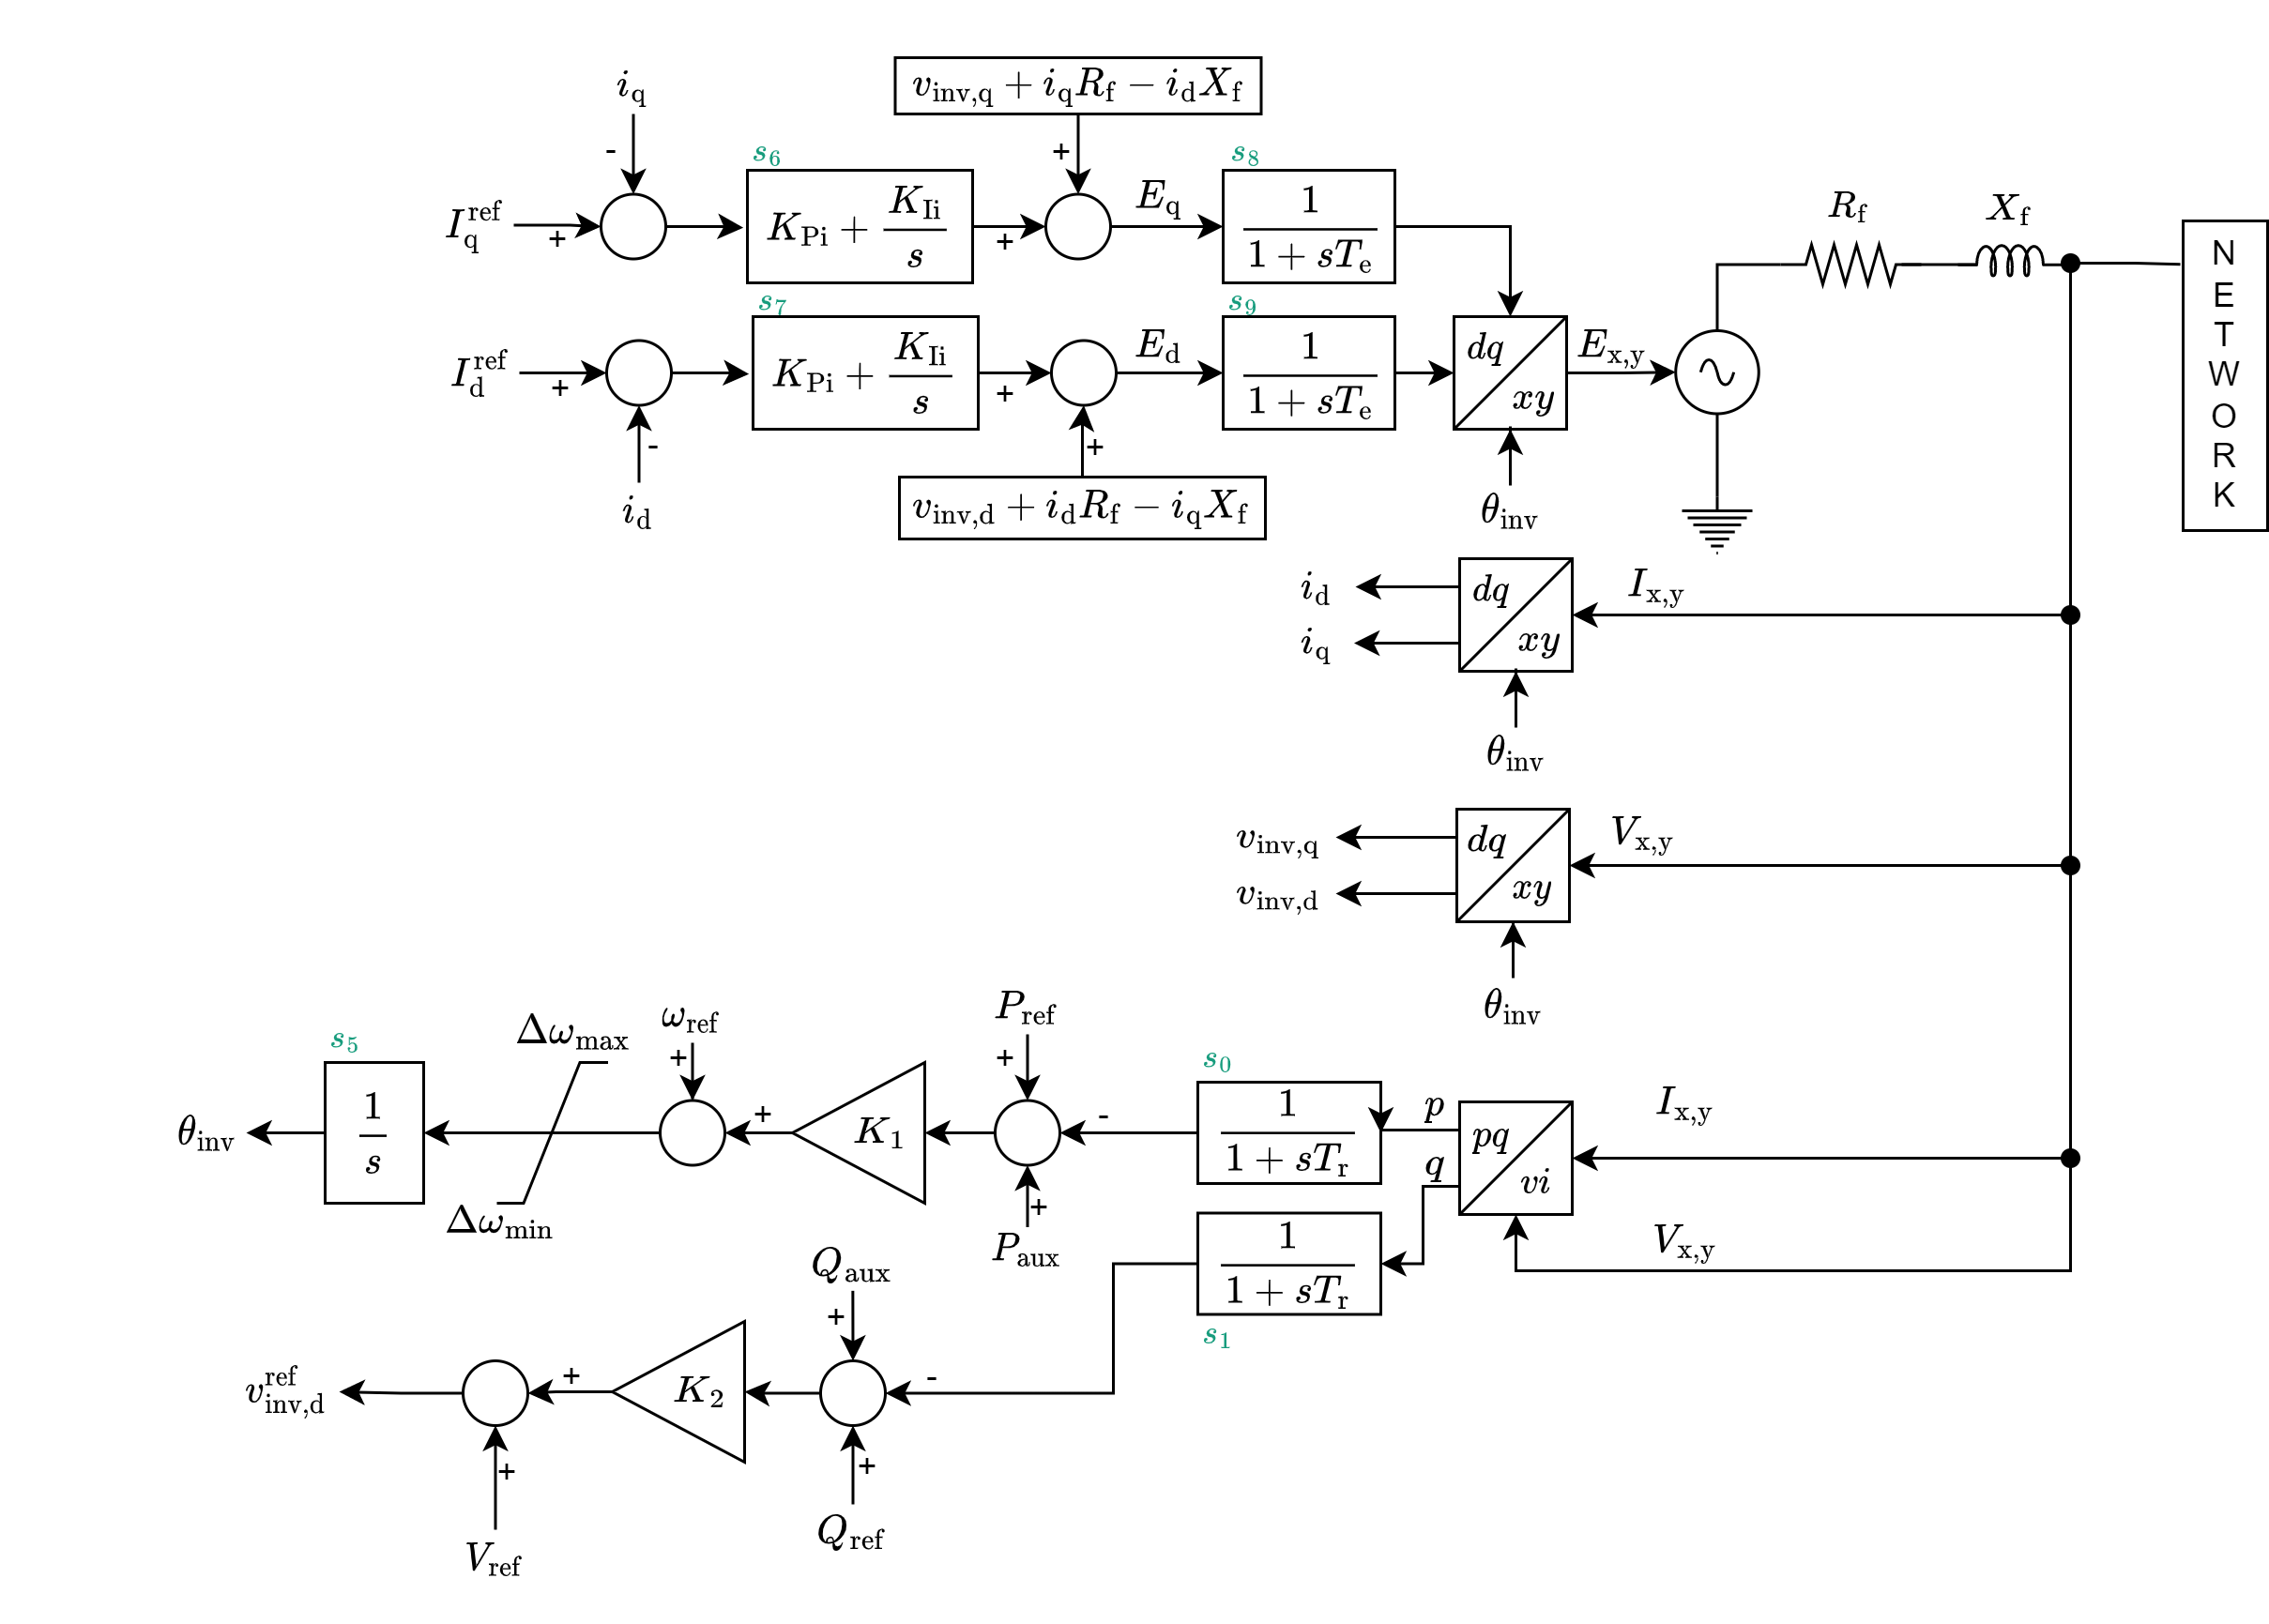
\includegraphics{./drawings/Droop_Mode.drawio.png}

}

\caption{\label{fig-droop_mode}Droop mode diagram}

\end{figure}%

\begin{figure}

\centering{

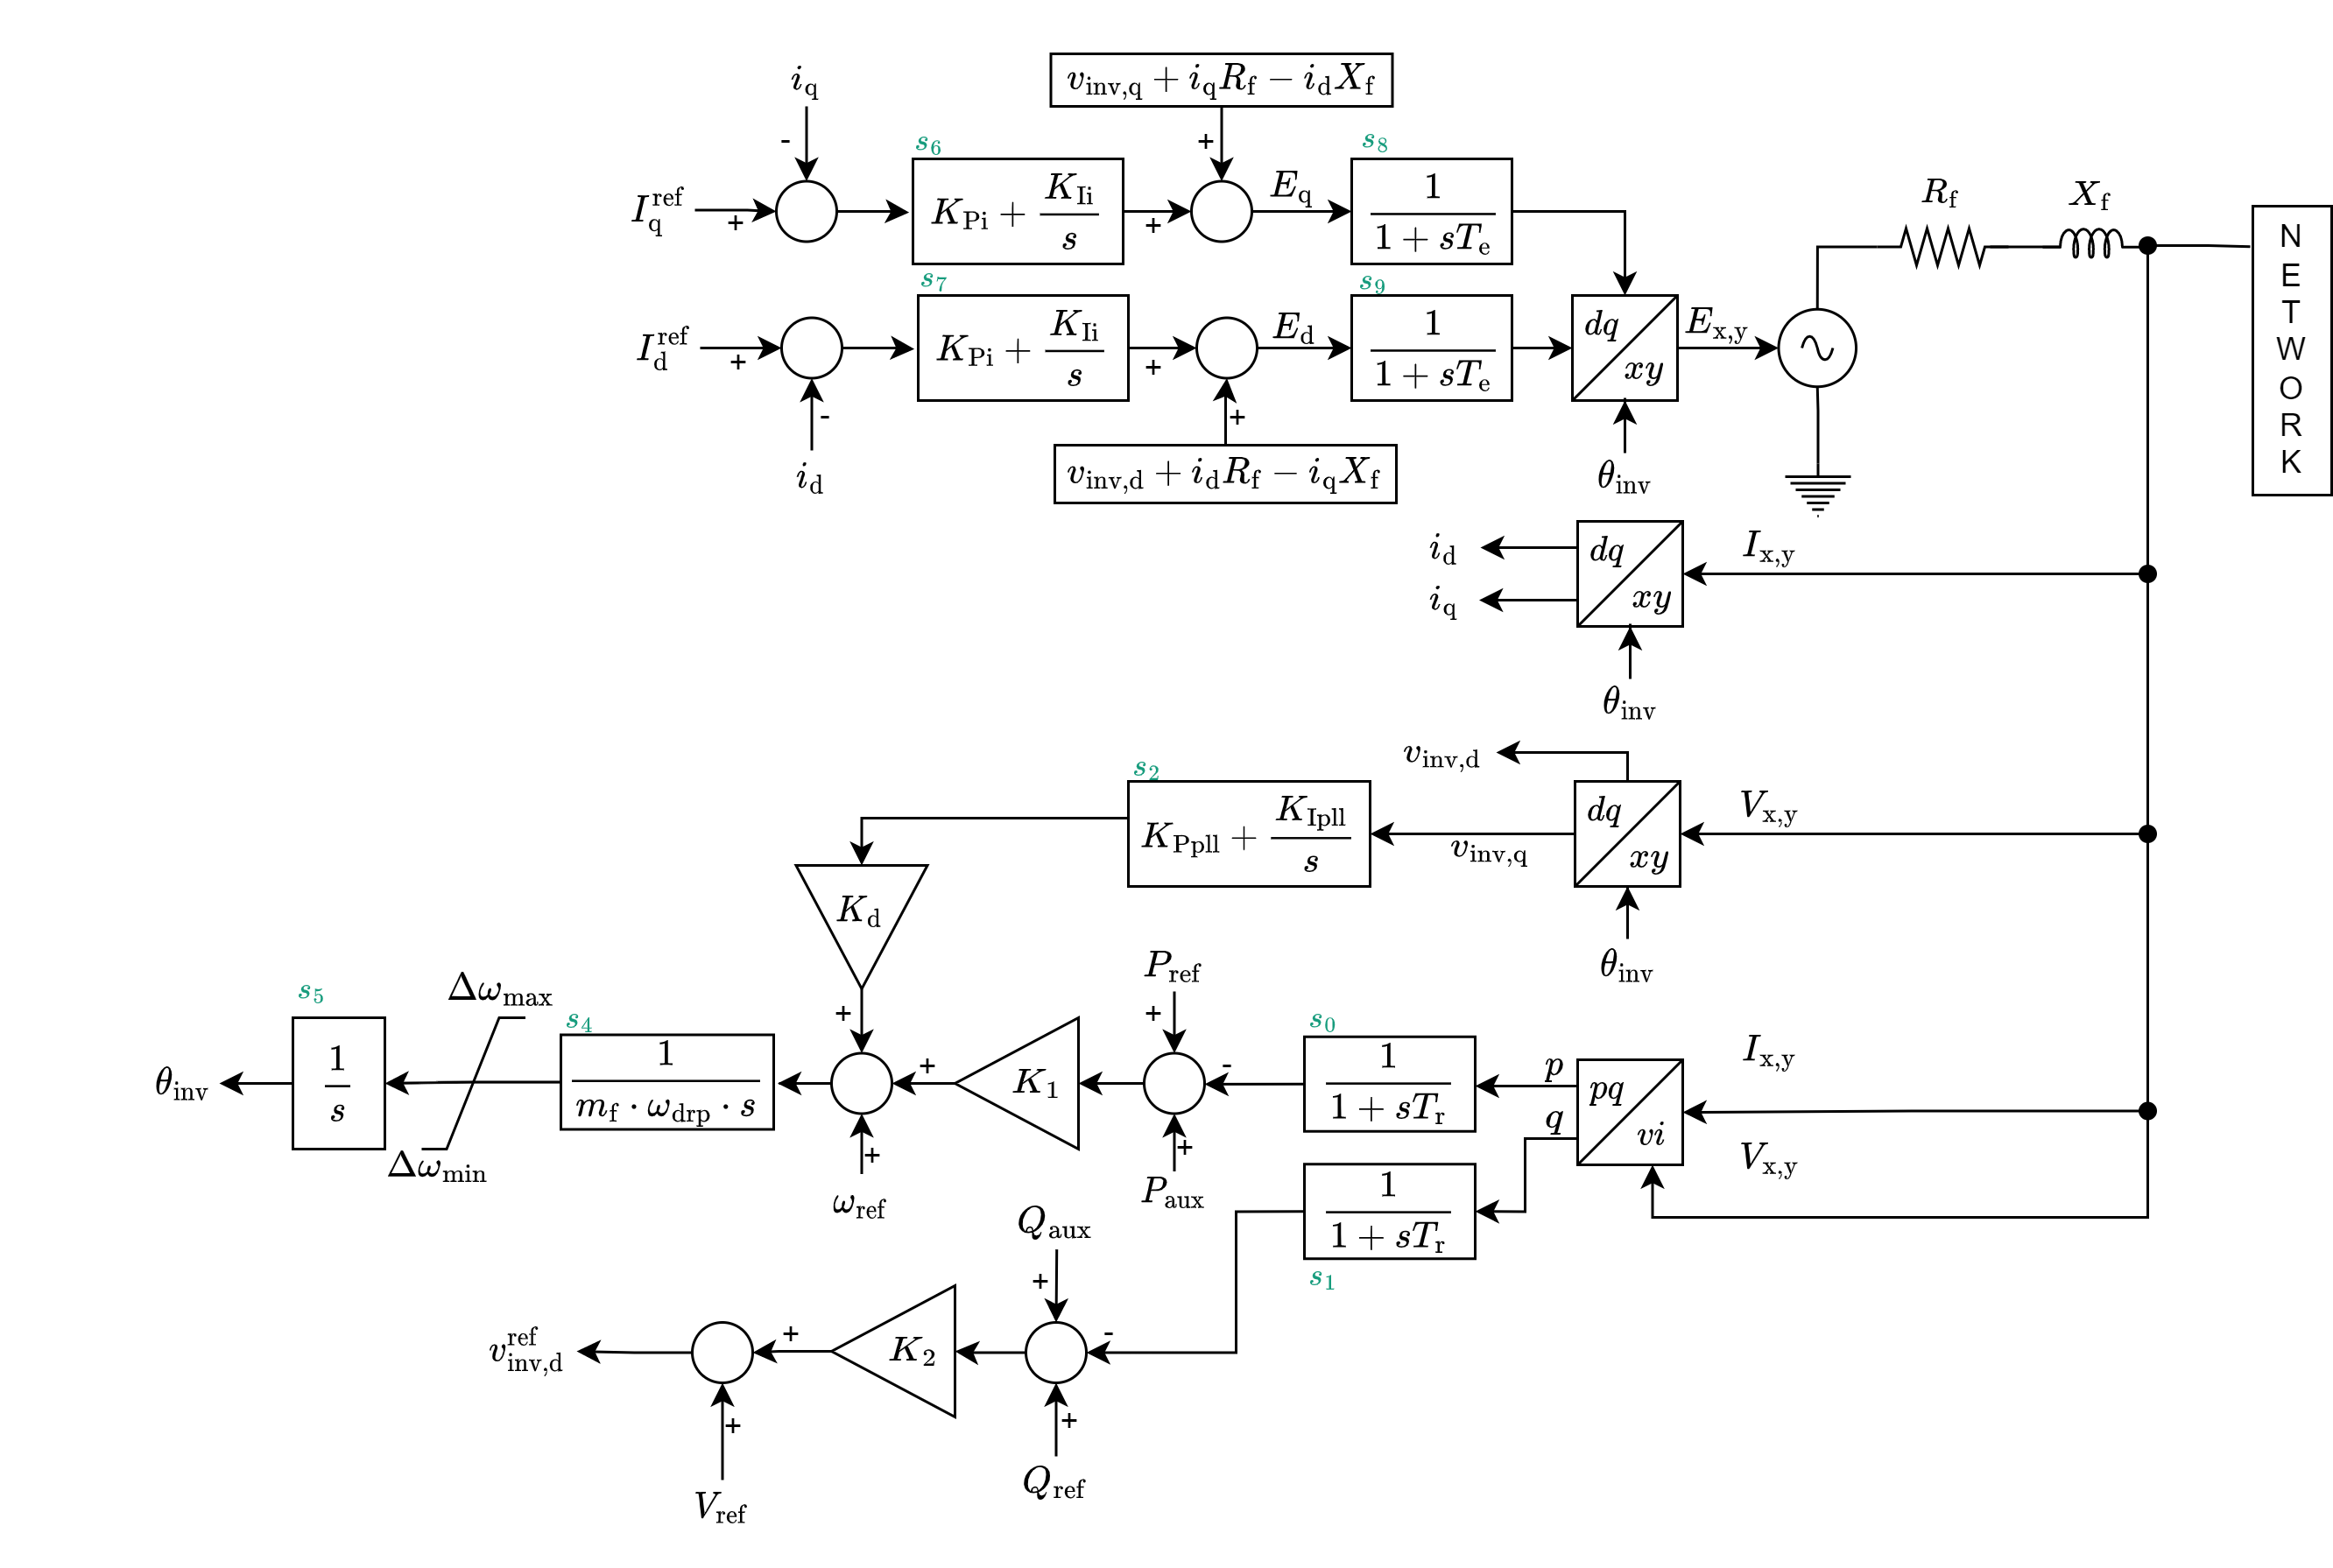
\includegraphics{./drawings/VSM_Mode.drawio.png}

}

\caption{\label{fig-vsm_mode}VSM mode diagram}

\end{figure}%

\begin{figure}

\centering{

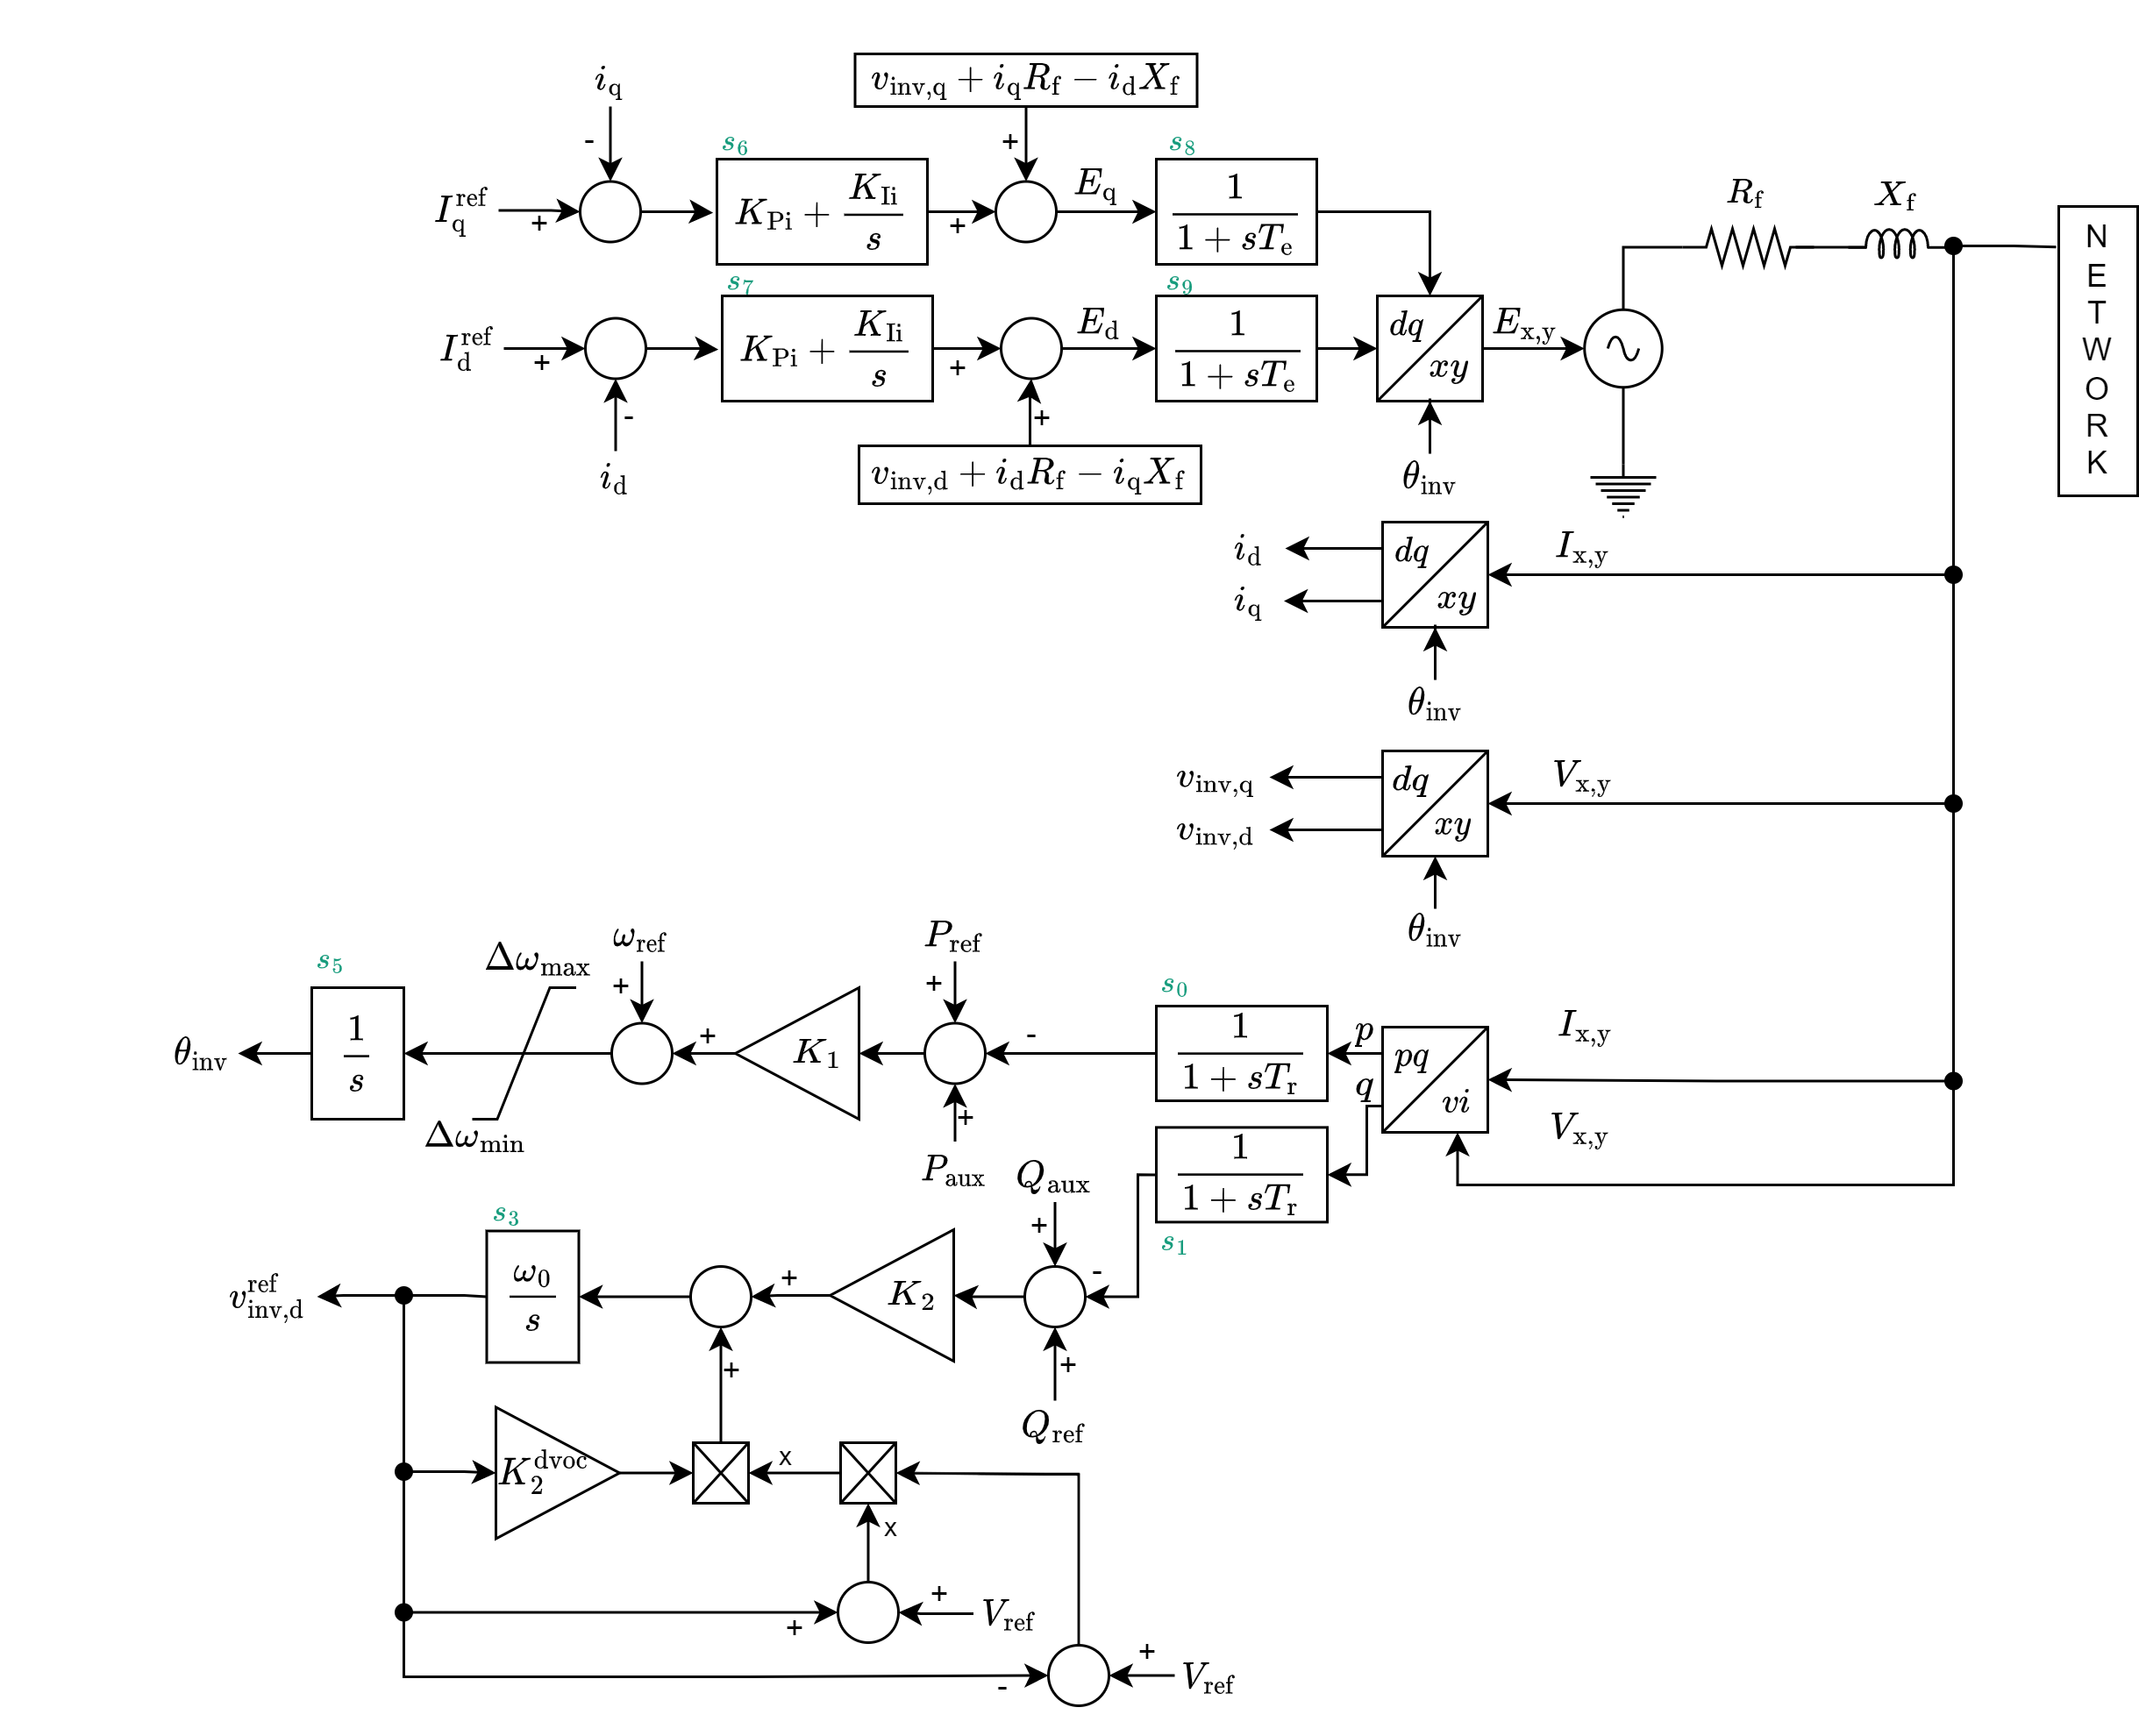
\includegraphics{./drawings/DVOC_Mode.drawio.png}

}

\caption{\label{fig-dvoc_mode}dVOC mode diagram}

\end{figure}%

\begin{figure}

\centering{

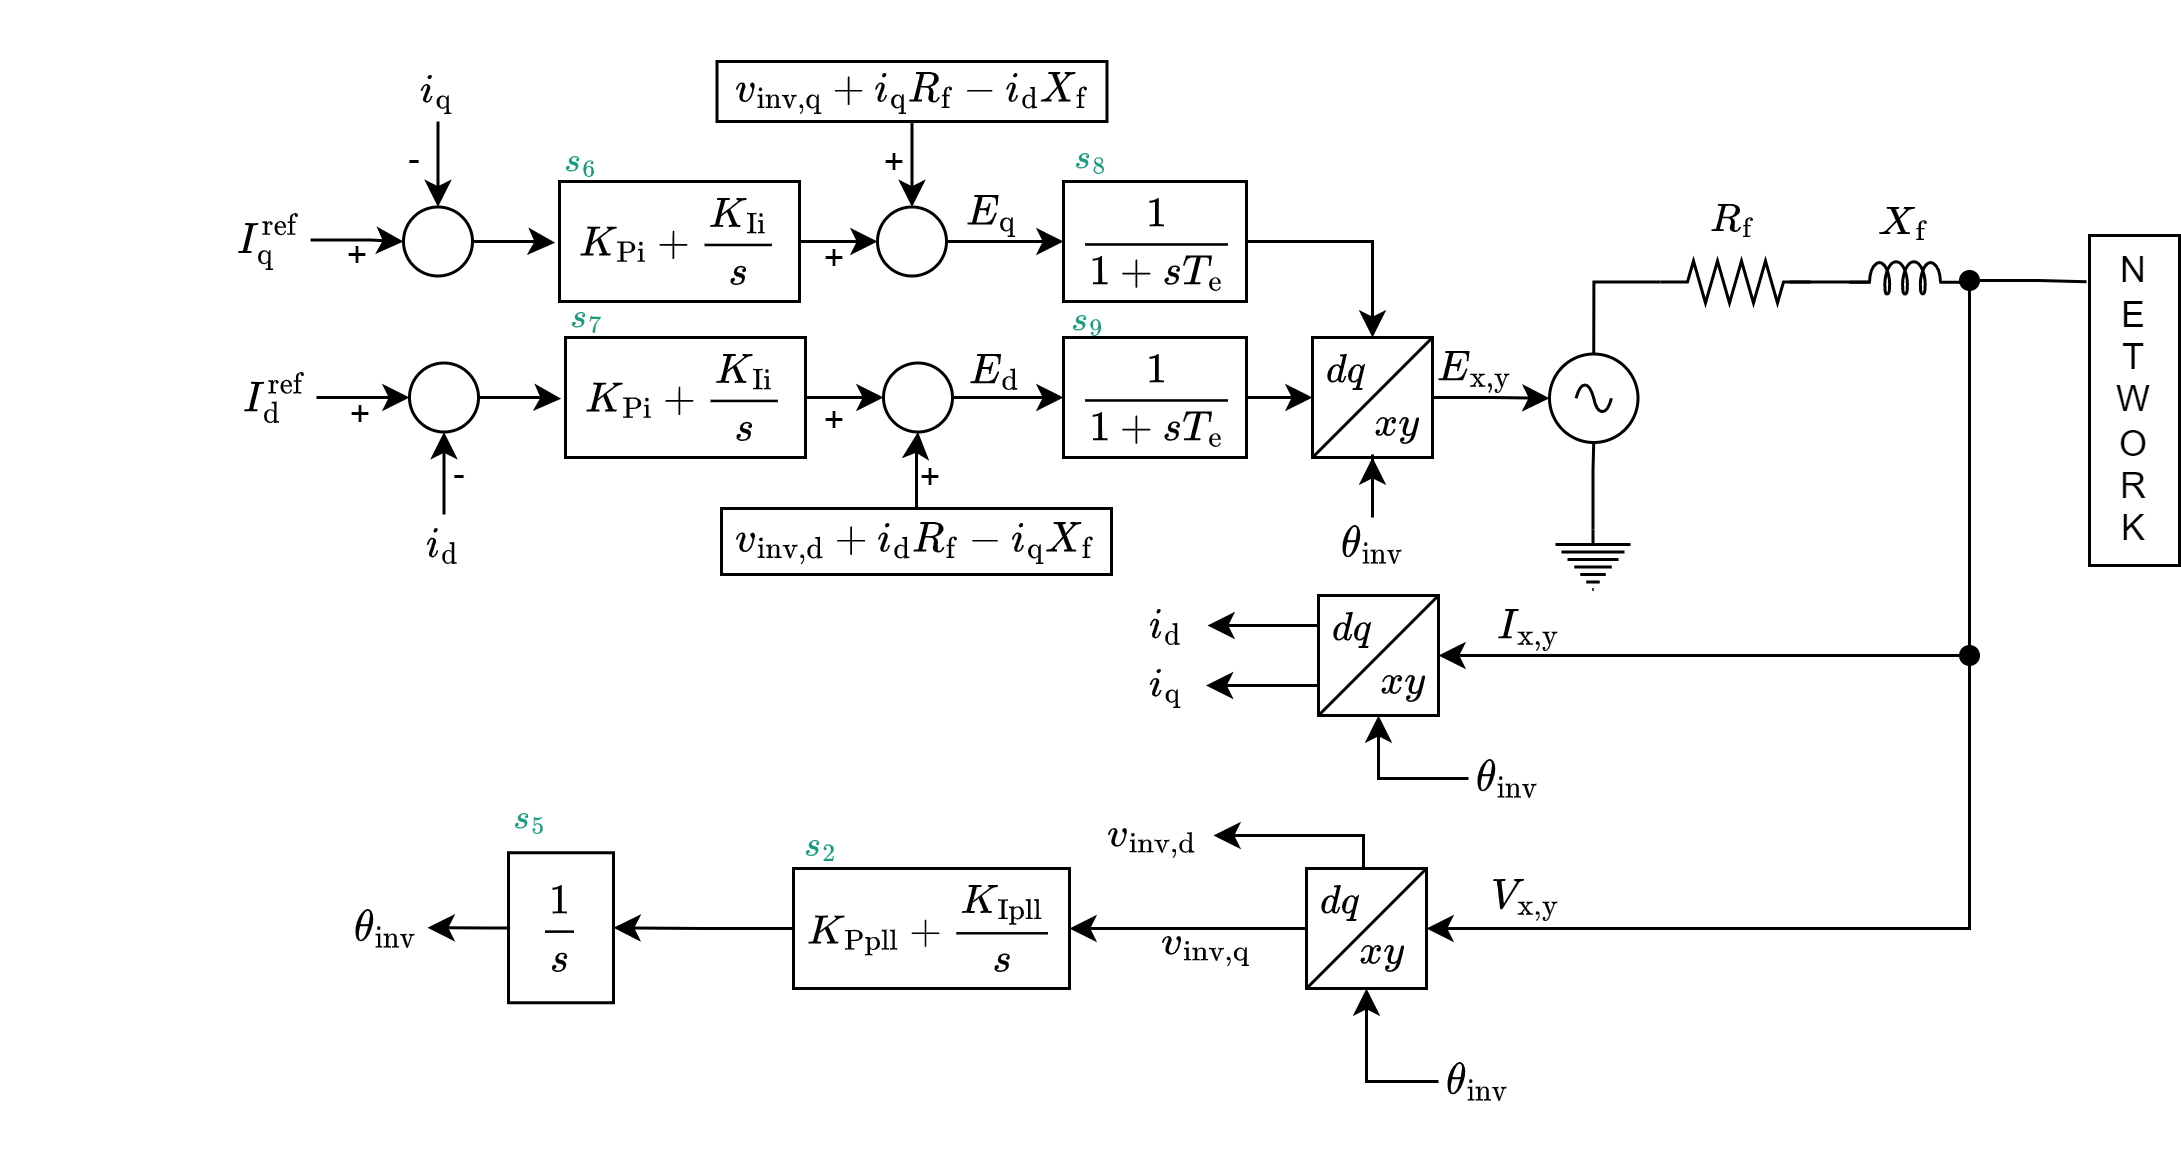
\includegraphics{./drawings/PLL_Mode.drawio.png}

}

\caption{\label{fig-pll_mode}PLL mode diagram}

\end{figure}%

\begin{tcolorbox}[enhanced jigsaw, colback=white, toprule=.15mm, leftrule=.75mm, colbacktitle=quarto-callout-note-color!10!white, colframe=quarto-callout-note-color-frame, breakable, opacityback=0, bottomrule=.15mm, opacitybacktitle=0.6, left=2mm, rightrule=.15mm, titlerule=0mm, bottomtitle=1mm, toptitle=1mm, coltitle=black, arc=.35mm, title=\textcolor{quarto-callout-note-color}{\faInfo}\hspace{0.5em}{Note}]

The xy reference frame is the real -- imaginary coordinate frame of the
network while the dq reference frame is the coordinate frame of the
control.The relative angle between these reference frames is denoted by
the control variable \(\theta_\mathrm{inv}\).

\end{tcolorbox}

\subsection{D and q reference currents
calculation}\label{d-and-q-reference-currents-calculation}

\begin{figure}

\centering{

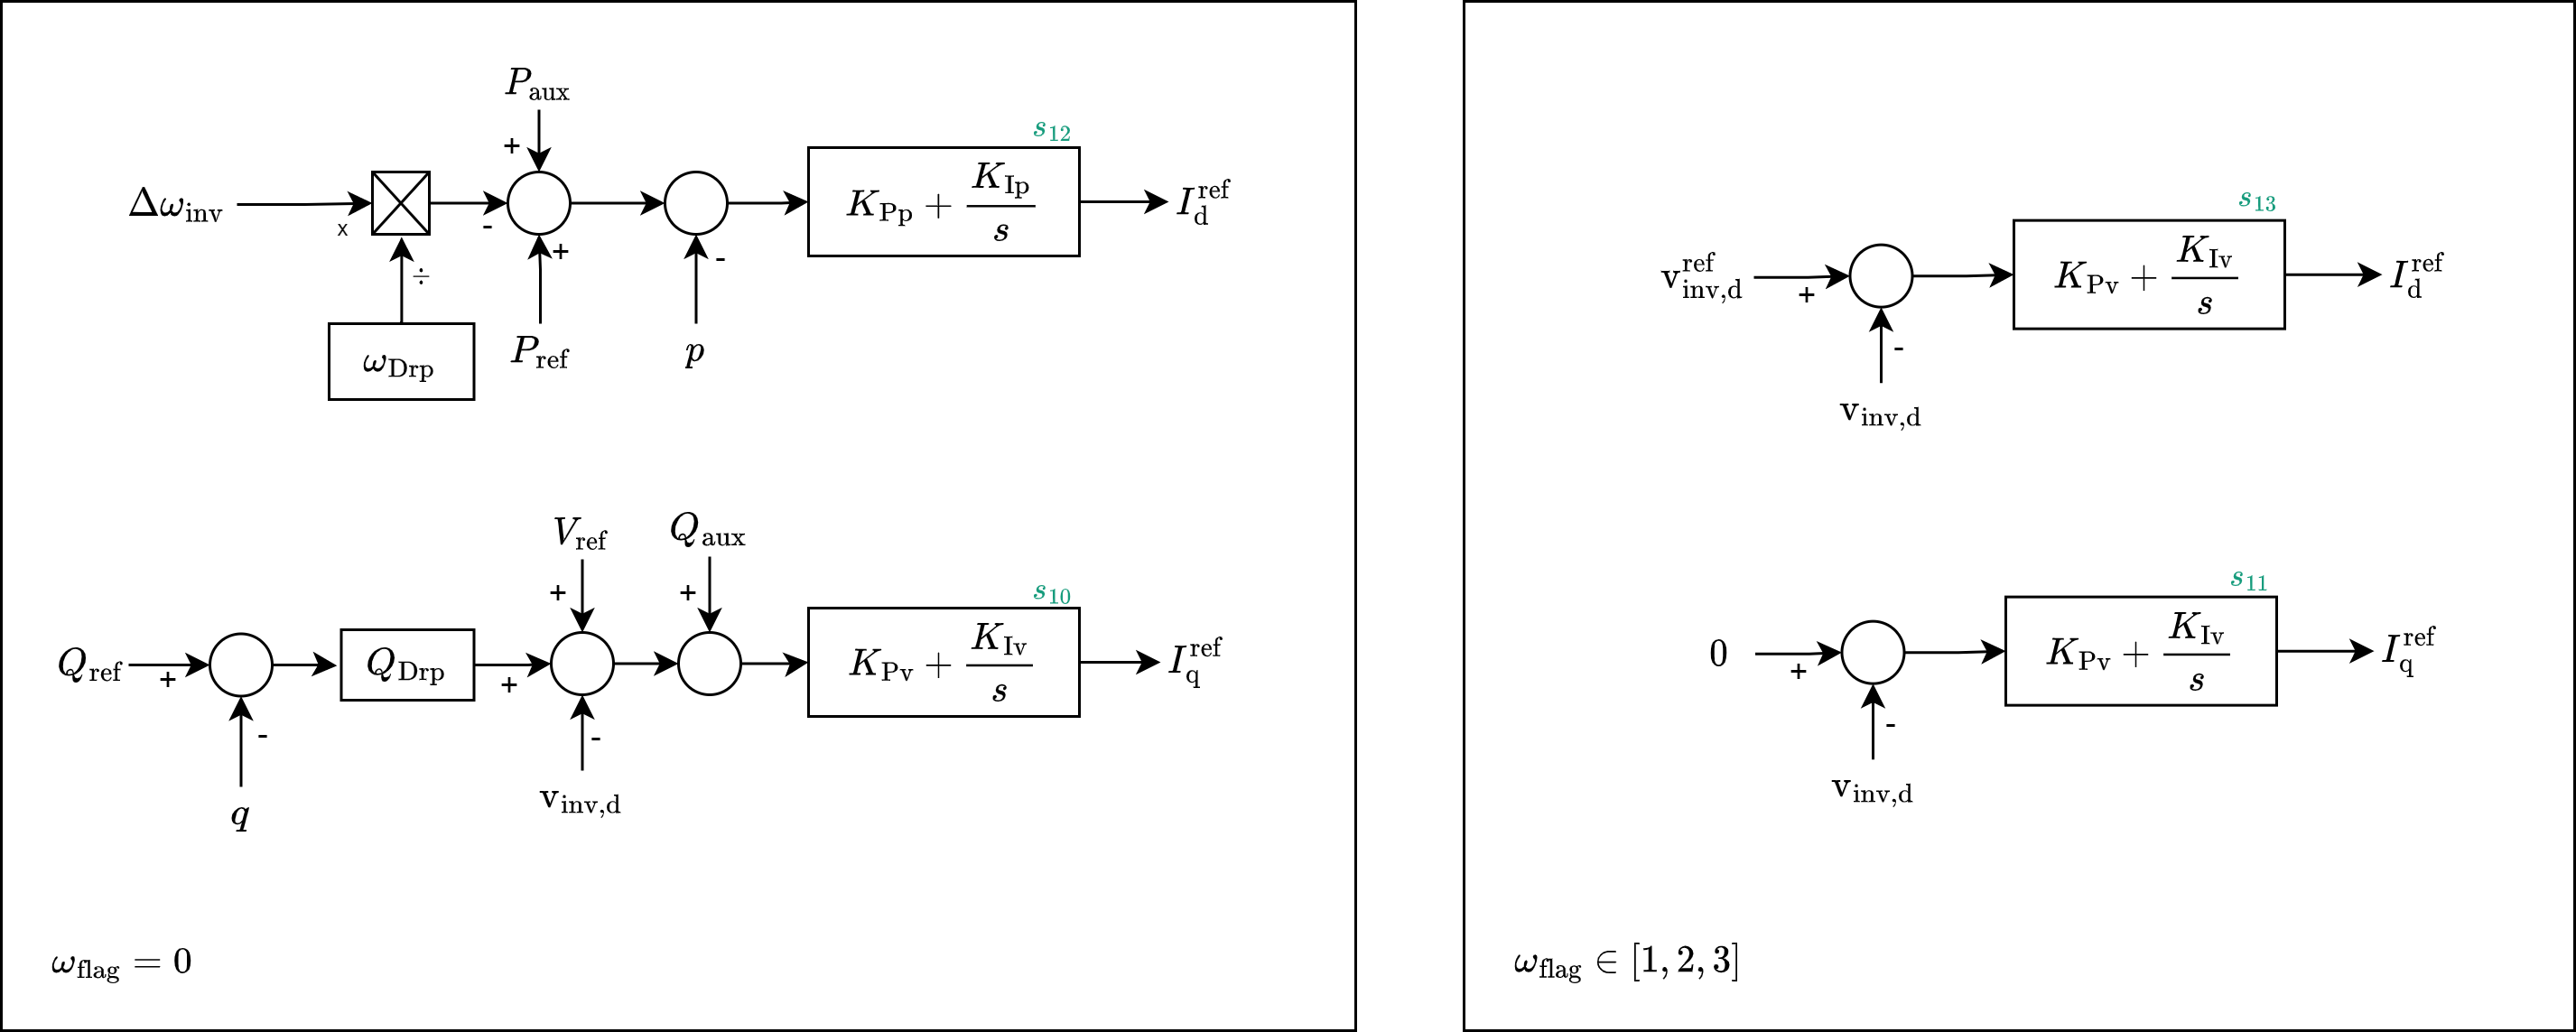
\includegraphics{./drawings/Grid_Forming.drawio.png}

}

\caption{\label{fig-IdIqRefCalculation}Calculation of d and q reference
currents}

\end{figure}%

\section{Parameters}\label{parameters}

Per-unit parameters are on base of \(P_\mathrm{base}\), which is
normally the capability of the inverter in MW.

\begin{longtable}[]{@{}
  >{\raggedright\arraybackslash}p{(\columnwidth - 10\tabcolsep) * \real{0.0600}}
  >{\raggedright\arraybackslash}p{(\columnwidth - 10\tabcolsep) * \real{0.0600}}
  >{\raggedright\arraybackslash}p{(\columnwidth - 10\tabcolsep) * \real{0.0500}}
  >{\raggedright\arraybackslash}p{(\columnwidth - 10\tabcolsep) * \real{0.1000}}
  >{\raggedright\arraybackslash}p{(\columnwidth - 10\tabcolsep) * \real{0.4400}}
  >{\raggedright\arraybackslash}p{(\columnwidth - 10\tabcolsep) * \real{0.1500}}@{}}
\caption{Parameters}\label{tbl-parameters}\tabularnewline
\toprule\noalign{}
\begin{minipage}[b]{\linewidth}\raggedright
name
\end{minipage} & \begin{minipage}[b]{\linewidth}\raggedright
type
\end{minipage} & \begin{minipage}[b]{\linewidth}\raggedright
unit
\end{minipage} & \begin{minipage}[b]{\linewidth}\raggedright
modelica name
\end{minipage} & \begin{minipage}[b]{\linewidth}\raggedright
description
\end{minipage} & \begin{minipage}[b]{\linewidth}\raggedright
typical value
\end{minipage} \\
\midrule\noalign{}
\endfirsthead
\toprule\noalign{}
\begin{minipage}[b]{\linewidth}\raggedright
name
\end{minipage} & \begin{minipage}[b]{\linewidth}\raggedright
type
\end{minipage} & \begin{minipage}[b]{\linewidth}\raggedright
unit
\end{minipage} & \begin{minipage}[b]{\linewidth}\raggedright
modelica name
\end{minipage} & \begin{minipage}[b]{\linewidth}\raggedright
description
\end{minipage} & \begin{minipage}[b]{\linewidth}\raggedright
typical value
\end{minipage} \\
\midrule\noalign{}
\endhead
\bottomrule\noalign{}
\endlastfoot
\(d_\mathrm{d}\) & float & pu & dd & VSM damping factor & 0.11 \\
\(K_\mathrm{Ip}\) & float & pu & Kpi & Active power integral gain &
20.0 \\
\(K_\mathrm{Pp}\) & float & pu & Kpp & Active power proportional gain &
0.5 \\
\(K_\mathrm{Iv}\) & float & pu & Kiv & Voltage control integral gain &
see Table~\ref{tbl-controllerParams} \\
\(K_\mathrm{Pv}\) & float & pu & Kpv & Voltage control proportional gain
& see Table~\ref{tbl-controllerParams} \\
\(K_\mathrm{Ii}\) & float & pu & Kii & Current controller integral gain
& 20.0 \\
\(K_\mathrm{Ipll}\) & float & pu & Ki & PLL integral gain & 700.0 \\
\(K_\mathrm{Pi}\) & float & pu & Kpi & Current controller proportional
gain & 0.5 \\
\(K_\mathrm{Ppll}\) & float & pu & Kp & PLL proportional gain & 20.0 \\
\(m_\mathrm{f}\) & float & pu & mf & VSM inertia constant & 0.15 \\
\(PQ_\mathrm{flag}\) & int & pu & PQflag & Current priority & 0 - P
prio.; 1 - Q-prio. \\
\(Q_\mathrm{drp}\) & float & pu & Qdroop & Voltage droop & 4.5 \\
\(R_\mathrm{f}\) & float & pu & RFilter & Filter resistance & 0.0015 \\
\(T_\mathrm{e}\) & float & s & te & Output state time constant & 0.01 \\
\(T_\mathrm{r}\) & float & s & tr & Transducer time constant & 0.005 \\
\(V_\mathrm{dip}\) & float & pu & Vdip & State freeze threshold & 0.8 \\
\(X_\mathrm{f}\) & float & pu & XFilter & Filter reactance & 0.15 \\
\(\Delta\omega_\mathrm{max}\) & float & rad/s & deltamax & Maximum
frequency deviation & 75.0/\(\omega_\mathrm{base}\) \\
\(\Delta\omega_\mathrm{min}\) & float & rad/s & deltamin & Minimum
frequency deviation & -75.0/\(\omega_\mathrm{base}\) \\
\(\omega_\mathrm{drp}\) & float & pu & wDroop & Frequency droop &
0.033 \\
\(\omega_\mathrm{flag}\) & int & pu & wflag & GFM control type & 0-3 \\
\(T\mathrm{f}\) & int & pu & tf & GFM control type & see
Table~\ref{tbl-controllerParams2} \\
\(T_\mathrm{v}\) & int & pu & tv & GFM control type & see
Table~\ref{tbl-controllerParams2} \\
\(K_\mathrm{1}\) & int & pu & k1 & GFM control type & see
Table~\ref{tbl-controllerParams2} \\
\(K\mathrm{2}\) & int & pu & k2 & GFM control type & see
Table~\ref{tbl-controllerParams2} \\
\(K_\mathrm{2}^{\mathrm{dvoc}}\) & int & pu & k2dvoc & GFM control type
& see Table~\ref{tbl-controllerParams2} \\
\end{longtable}

\(\omega_\mathrm{base}\) is the nominal angular frequency in rad/s.

\begin{longtable}[]{@{}
  >{\raggedright\arraybackslash}p{(\columnwidth - 4\tabcolsep) * \real{0.2174}}
  >{\raggedright\arraybackslash}p{(\columnwidth - 4\tabcolsep) * \real{0.3478}}
  >{\raggedright\arraybackslash}p{(\columnwidth - 4\tabcolsep) * \real{0.4348}}@{}}
\caption{Voltage controller parameters depending on control
mode}\label{tbl-controllerParams}\tabularnewline
\toprule\noalign{}
\begin{minipage}[b]{\linewidth}\raggedright
name
\end{minipage} & \begin{minipage}[b]{\linewidth}\raggedright
\(\omega_\mathrm{flag}=0\)
\end{minipage} & \begin{minipage}[b]{\linewidth}\raggedright
\(\omega_\mathrm{flag} \neq  0\)
\end{minipage} \\
\midrule\noalign{}
\endfirsthead
\toprule\noalign{}
\begin{minipage}[b]{\linewidth}\raggedright
name
\end{minipage} & \begin{minipage}[b]{\linewidth}\raggedright
\(\omega_\mathrm{flag}=0\)
\end{minipage} & \begin{minipage}[b]{\linewidth}\raggedright
\(\omega_\mathrm{flag} \neq  0\)
\end{minipage} \\
\midrule\noalign{}
\endhead
\bottomrule\noalign{}
\endlastfoot
\(K_\mathrm{Iv}\) & 150.0 & 10.0 \\
\(K_\mathrm{Pv}\) & 0.5 & 3.0 \\
\end{longtable}

\begin{longtable}[]{@{}
  >{\raggedright\arraybackslash}p{(\columnwidth - 8\tabcolsep) * \real{0.2000}}
  >{\raggedright\arraybackslash}p{(\columnwidth - 8\tabcolsep) * \real{0.1000}}
  >{\raggedright\arraybackslash}p{(\columnwidth - 8\tabcolsep) * \real{0.1000}}
  >{\raggedright\arraybackslash}p{(\columnwidth - 8\tabcolsep) * \real{0.1000}}
  >{\raggedright\arraybackslash}p{(\columnwidth - 8\tabcolsep) * \real{0.1000}}@{}}
\caption{Mode dependent
paramaters}\label{tbl-controllerParams2}\tabularnewline
\toprule\noalign{}
\begin{minipage}[b]{\linewidth}\raggedright
GFM Control
\end{minipage} & \begin{minipage}[b]{\linewidth}\raggedright
\(K_\mathrm{d}\)
\end{minipage} & \begin{minipage}[b]{\linewidth}\raggedright
\(K_\mathrm{1}\)
\end{minipage} & \begin{minipage}[b]{\linewidth}\raggedright
\(K_\mathrm{2}\)
\end{minipage} & \begin{minipage}[b]{\linewidth}\raggedright
\(K_\mathrm{2}^{\mathrm{dVOC}}\)
\end{minipage} \\
\midrule\noalign{}
\endfirsthead
\toprule\noalign{}
\begin{minipage}[b]{\linewidth}\raggedright
GFM Control
\end{minipage} & \begin{minipage}[b]{\linewidth}\raggedright
\(K_\mathrm{d}\)
\end{minipage} & \begin{minipage}[b]{\linewidth}\raggedright
\(K_\mathrm{1}\)
\end{minipage} & \begin{minipage}[b]{\linewidth}\raggedright
\(K_\mathrm{2}\)
\end{minipage} & \begin{minipage}[b]{\linewidth}\raggedright
\(K_\mathrm{2}^{\mathrm{dVOC}}\)
\end{minipage} \\
\midrule\noalign{}
\endhead
\bottomrule\noalign{}
\endlastfoot
PLL & 0.0 & 0.0 & 0.0 & 0.0 \\
Droop & 0.0 & \(\omega_\mathrm{drp}\) & \(Q_\mathrm{drp}\) & 0.0 \\
VSM & \(d_\mathrm{d}\omega_\mathrm{{drp}}\) & \(\omega_\mathrm{drp}\) &
\(Q_\mathrm{drp}\) & 0.0 \\
dVOC & 0.0 & \(\omega_\mathrm{drp}/s_2^3\) & \(\omega_\mathrm{drp}/s_3\)
& see Equation~\ref{eq-dvoc1} \\
\end{longtable}

\begin{equation}\phantomsection\label{eq-dvoc1}{
\frac{K_2^{dvoc}}{\omega_{drp}} = \frac{4 \cdot 100^4}{100^4 - \left( 2 \cdot \left(100 - 100 \cdot Q_{drp}\right)^2 - 100^2 \right)^2}
}\end{equation}

\subsection{Inputs}\label{inputs}

\begin{longtable}[]{@{}
  >{\raggedright\arraybackslash}p{(\columnwidth - 8\tabcolsep) * \real{0.2500}}
  >{\raggedright\arraybackslash}p{(\columnwidth - 8\tabcolsep) * \real{0.0595}}
  >{\raggedright\arraybackslash}p{(\columnwidth - 8\tabcolsep) * \real{0.0476}}
  >{\raggedright\arraybackslash}p{(\columnwidth - 8\tabcolsep) * \real{0.1548}}
  >{\raggedright\arraybackslash}p{(\columnwidth - 8\tabcolsep) * \real{0.4881}}@{}}
\caption{Inputs}\label{tbl-inputs}\tabularnewline
\toprule\noalign{}
\begin{minipage}[b]{\linewidth}\raggedright
name
\end{minipage} & \begin{minipage}[b]{\linewidth}\raggedright
type
\end{minipage} & \begin{minipage}[b]{\linewidth}\raggedright
unit
\end{minipage} & \begin{minipage}[b]{\linewidth}\raggedright
modelica name
\end{minipage} & \begin{minipage}[b]{\linewidth}\raggedright
description
\end{minipage} \\
\midrule\noalign{}
\endfirsthead
\toprule\noalign{}
\begin{minipage}[b]{\linewidth}\raggedright
name
\end{minipage} & \begin{minipage}[b]{\linewidth}\raggedright
type
\end{minipage} & \begin{minipage}[b]{\linewidth}\raggedright
unit
\end{minipage} & \begin{minipage}[b]{\linewidth}\raggedright
modelica name
\end{minipage} & \begin{minipage}[b]{\linewidth}\raggedright
description
\end{minipage} \\
\midrule\noalign{}
\endhead
\bottomrule\noalign{}
\endlastfoot
\(V_\mathrm{ref}\) & float & pu & VRefPu & voltage setpoint \\
\(\omega_\mathrm{ref}\) & float & pu & deltaOmega & speed reference
(difference to nominal) \\
\(Q_\mathrm{ref}\) & float & pu & QRefPu & reactive power setpoint \\
\(P_\mathrm{ref}\) & float & pu & PRefPu & active power setpoint \\
\(Q_\mathrm{aux}\) & float & pu & QAuxPu & auxiliary reactive power \\
\(P_\mathrm{aux}\) & float & pu & PAuxPu & auxiliary active power \\
\(V_\mathrm{x,y}\) & float & pu & uINjPu & measured voltage in
real/imag. quantities \\
\(I_\mathrm{x,y}\) & float & pu & iINjPu & measured current in
real/imag. quantities \\
\end{longtable}

\subsection{Outputs}\label{outputs}

\begin{longtable}[]{@{}
  >{\raggedright\arraybackslash}p{(\columnwidth - 8\tabcolsep) * \real{0.2059}}
  >{\raggedright\arraybackslash}p{(\columnwidth - 8\tabcolsep) * \real{0.0735}}
  >{\raggedright\arraybackslash}p{(\columnwidth - 8\tabcolsep) * \real{0.0588}}
  >{\raggedright\arraybackslash}p{(\columnwidth - 8\tabcolsep) * \real{0.1912}}
  >{\raggedright\arraybackslash}p{(\columnwidth - 8\tabcolsep) * \real{0.4706}}@{}}
\caption{Outputs}\label{tbl-outputs}\tabularnewline
\toprule\noalign{}
\begin{minipage}[b]{\linewidth}\raggedright
name
\end{minipage} & \begin{minipage}[b]{\linewidth}\raggedright
type
\end{minipage} & \begin{minipage}[b]{\linewidth}\raggedright
unit
\end{minipage} & \begin{minipage}[b]{\linewidth}\raggedright
modelica name
\end{minipage} & \begin{minipage}[b]{\linewidth}\raggedright
description
\end{minipage} \\
\midrule\noalign{}
\endfirsthead
\toprule\noalign{}
\begin{minipage}[b]{\linewidth}\raggedright
name
\end{minipage} & \begin{minipage}[b]{\linewidth}\raggedright
type
\end{minipage} & \begin{minipage}[b]{\linewidth}\raggedright
unit
\end{minipage} & \begin{minipage}[b]{\linewidth}\raggedright
modelica name
\end{minipage} & \begin{minipage}[b]{\linewidth}\raggedright
description
\end{minipage} \\
\midrule\noalign{}
\endhead
\bottomrule\noalign{}
\endlastfoot
\(E_\mathrm{x}\) & float & pu & urScourePu & output voltage in real
quantity \\
\(E_\mathrm{y}\) & float & pu & uiScourePu & output voltage in imag
quantity \\
\end{longtable}

\section{Initial equations}\label{initial-equations}

\begin{equation}\phantomsection\label{eq-s0}{
s_0 = P_\mathrm{ref}
}\end{equation}

\begin{equation}\phantomsection\label{eq-s1}{
s_1 = Q_\mathrm{ref}
}\end{equation}

\begin{equation}\phantomsection\label{eq-s2}{ 
s_2 = \theta_\mathrm{loadflow} 
}\end{equation} \begin{equation}\phantomsection\label{eq-s3}{ 
s_3 = V_\mathrm{ref}
}\end{equation} \begin{equation}\phantomsection\label{eq-s4}{ 
s_4 = \omega_\mathrm{grid} - \omega_\mathrm{base}
}\end{equation} \begin{equation}\phantomsection\label{eq-s5}{ 
s_5 = \theta_\mathrm{loadflow} 
}\end{equation} \begin{equation}\phantomsection\label{eq-s6}{ 
s_6 = E_\mathrm{q,loadflow} - v_\mathrm{q,loadflow} - i_\mathrm{q,loadflow}R_\mathrm{f} - i_\mathrm{d,loadflow}X_\mathrm{f}
}\end{equation} \begin{equation}\phantomsection\label{eq-s7}{ 
s_7 = E_\mathrm{d,loadflow} - v_\mathrm{d,loadflow} - i_\mathrm{d,loadflow}R_\mathrm{f} + i_\mathrm{q,loadflow}X_\mathrm{f}
}\end{equation} \begin{equation}\phantomsection\label{eq-s8}{ 
s_8 = E_\mathrm{q,loadflow} 
}\end{equation} \begin{equation}\phantomsection\label{eq-s9}{ 
s_9 = E_\mathrm{d,loadflow} 
}\end{equation}

\begin{equation}\phantomsection\label{eq-s10}{ 
s_{10} = i_\mathrm{q,loadflow} 
}\end{equation} \begin{equation}\phantomsection\label{eq-s11}{ 
s_{11} = i_\mathrm{q,loadflow} 
}\end{equation} \begin{equation}\phantomsection\label{eq-s12}{ 
s_{12} = i_\mathrm{d,loadflow}  
}\end{equation} \begin{equation}\phantomsection\label{eq-s13}{ 
s_{13} = i_\mathrm{d,loadflow} 
}\end{equation}

The index ``loadflow'' indicates that this is the solution of a
loadflow.

\section{Assumptions in modelica implementation (Open source
implementations)}\label{assumptions-in-modelica-implementation-open-source-implementations}

In GFM mode the output angle is multiplied with the nominal angular
freauency in rad/s (\(\omega_\mathrm{base}\)). \(\omega_\mathrm{ref}\)
is set to zero as the whole model is already in real/imaginary
quantities. In case of a speed reference change only the difference to
nominal speed has to be given.

\section{Table of references \&
license}\label{table-of-references-license}

\phantomsection\label{refs}
\begin{CSLReferences}{0}{0}
\bibitem[\citeproctext]{ref-epri2021}
\CSLLeftMargin{{[}1{]} }%
\CSLRightInline{EPRI, {``Generic {Positive Sequence Domain Model} of
{Grid Forming Inverter Based Resource},''} Dec. 2021.}

\end{CSLReferences}




\end{document}
